\begin{frame}[t,squeeze,allowframebreaks, allowdisplaybreaks]
    \frametitle{B-Tree Operations---Delete (Example)}
    \newcounter{delete-example}
    \newcounter{delete-img-example}
    \newcounter{delete-step-example}[delete-example]
    \setcounter{delete-example}{0}
    \setcounter{delete-img-example}{0}
    \setcounter{delete-step-example}{0}
    % Delete 1
    \stepcounter{delete-example}
    \stepcounter{delete-img-example}
	\stepcounter{delete-step-example}
    \begin{columns}
        \begin{column}{.47\textwidth}
            \inputminted[%
                highlightlines={1,5,6},%
                firstline=1,%
                lastline=6,%
                tabsize=1,%
                fontsize=\examplefnt,%
            ]{c}{resources/code/b_tree_delete.c}
        \end{column}
        \begin{column}{.5\textwidth}
            \examplefnt{%
                \begin{itemize}
                    \item Delete \arabic{delete-example}; Step \arabic{delete-step-example};
                    \item \hlght{tree=(*pag 0); delete\_key=32;}
                    \item finished;
                    \item i; j;
                    \item current=(*pag 0); tmp\_node;
                \end{itemize}
            }
        \end{column}
    \end{columns}
    \begin{figure}[h!]
        \includegraphics[%
            height=0.5\textheight,%
            page=\value{delete-img-example},%
        ]{resources/made/B-Trees_delete_example.pdf}
    \end{figure}
    \framebreak{}
    \stepcounter{delete-img-example}
	\stepcounter{delete-step-example}
    \begin{columns}
        \begin{column}{.47\textwidth}
            \inputminted[%
                highlightlines={11,12},%
                firstline=7,%
                lastline=12,%
                tabsize=1,%
                fontsize=\examplefnt,%
            ]{c}{resources/code/b_tree_delete.c}
        \end{column}
        \begin{column}{.5\textwidth}
            \examplefnt{%
                \begin{itemize}
                    \item Delete \arabic{delete-example}; Step \arabic{delete-step-example};
                    \item tree=(*pag 0); delete\_key=32;
                    \item finished;
                    \item i; j;
                    \item current=(*pag 0); tmp\_node;
                    \item \hlght{lower=0; upper=2;}
                \end{itemize}
            }
        \end{column}
    \end{columns}
    \begin{figure}[h!]
        \includegraphics[%
            height=0.5\textheight,%
            page=\value{delete-img-example},%
        ]{resources/made/B-Trees_delete_example.pdf}
    \end{figure}
    \framebreak{}
    \stepcounter{delete-img-example}
	\stepcounter{delete-step-example}
    \begin{columns}
        \begin{column}{.47\textwidth}
            \inputminted[%
                highlightlines={13,14,15},%
                firstline=13,%
                lastline=18,%
                tabsize=1,%
                fontsize=\examplefnt,%
            ]{c}{resources/code/b_tree_delete.c}
        \end{column}
        \begin{column}{.5\textwidth}
            \examplefnt{%
                \begin{itemize}
                    \item Delete \arabic{delete-example}; Step \arabic{delete-step-example};
                    \item tree=(*pag 0); delete\_key=32;
                    \item finished;
                    \item i; j;
                    \item current=(*pag 0); tmp\_node;
                    \item lower=0; \hlght{upper=2 \rarr{} 1;}
                \end{itemize}
            }
        \end{column}
    \end{columns}
    \begin{figure}[h!]
        \includegraphics[%
            height=0.5\textheight,%
            page=\value{delete-img-example},%
        ]{resources/made/B-Trees_delete_example.pdf}
    \end{figure}
    \framebreak{}
    \stepcounter{delete-img-example}
	\stepcounter{delete-step-example}
    \begin{columns}
        \begin{column}{.47\textwidth}
            \inputminted[%
                highlightlines={7},%
                firstline=7,%
                lastline=7,%
                tabsize=1,%
                fontsize=\examplefnt,%
            ]{c}{resources/code/b_tree_delete.c}
            \inputminted[%
                highlightlines={13},%
                firstline=13,%
                lastline=13,%
                tabsize=1,%
                fontsize=\examplefnt,%
            ]{c}{resources/code/b_tree_delete.c}
            \inputminted[%
                highlightlines={20,21,22},%
                firstline=20,%
                lastline=23,%
                tabsize=1,%
                fontsize=\examplefnt,%
            ]{c}{resources/code/b_tree_delete.c}
        \end{column}
        \begin{column}{.5\textwidth}
            \examplefnt{%
                \begin{itemize}
                    \item Delete \arabic{delete-example}; Step \arabic{delete-step-example};
                    \item tree=(*pag 0); delete\_key=32;
                    \item finished;
                    \item i; j;
                    \item \hlght{current=(*pag 0) \rarr{} (*pag 6)}; tmp\_node;
                    \item \hlght{lower=0; upper=1;}
                \end{itemize}
            }
        \end{column}
    \end{columns}
    \begin{figure}[h!]
        \includegraphics[%
            height=0.5\textheight,%
            page=\value{delete-img-example},%
        ]{resources/made/B-Trees_delete_example.pdf}
    \end{figure}
    \framebreak{}
    \stepcounter{delete-img-example}
	\stepcounter{delete-step-example}
    \begin{columns}
        \begin{column}{.47\textwidth}
            \inputminted[%
                highlightlines={11,12},%
                firstline=7,%
                lastline=12,%
                tabsize=1,%
                fontsize=\examplefnt,%
            ]{c}{resources/code/b_tree_delete.c}
        \end{column}
        \begin{column}{.5\textwidth}
            \examplefnt{%
                \begin{itemize}
                    \item Delete \arabic{delete-example}; Step \arabic{delete-step-example};
                    \item tree=(*pag 0); delete\_key=32;
                    \item finished;
                    \item i; j;
                    \item current=(*pag 6); tmp\_node;
                    \item \hlght{lower=0; upper=2;}
                \end{itemize}
            }
        \end{column}
    \end{columns}
    \begin{figure}[h!]
        \includegraphics[%
            height=0.5\textheight,%
            page=\value{delete-img-example},%
        ]{resources/made/B-Trees_delete_example.pdf}
    \end{figure}
    \framebreak{}
    \stepcounter{delete-img-example}
	\stepcounter{delete-step-example}
    \begin{columns}
        \begin{column}{.47\textwidth}
            \inputminted[%
                highlightlines={13,14,17},%
                firstline=13,%
                lastline=18,%
                tabsize=1,%
                fontsize=\examplefnt,%
            ]{c}{resources/code/b_tree_delete.c}
        \end{column}
        \begin{column}{.5\textwidth}
            \examplefnt{%
                \begin{itemize}
                    \item Delete \arabic{delete-example}; Step \arabic{delete-step-example};
                    \item tree=(*pag 0); delete\_key=32;
                    \item finished;
                    \item i; j;
                    \item current=(*pag 6); tmp\_node;
                    \item \hlght{lower=0 \rarr{} 1; upper=2;}
                \end{itemize}
            }
        \end{column}
    \end{columns}
    \begin{figure}[h!]
        \includegraphics[%
            height=0.5\textheight,%
            page=\value{delete-img-example},%
        ]{resources/made/B-Trees_delete_example.pdf}
    \end{figure}
    \framebreak{}
    \stepcounter{delete-img-example}
	\stepcounter{delete-step-example}
    \begin{columns}
        \begin{column}{.47\textwidth}
            \inputminted[%
                highlightlines={7},%
                firstline=7,%
                lastline=7,%
                tabsize=1,%
                fontsize=\examplefnt,%
            ]{c}{resources/code/b_tree_delete.c}
            \inputminted[%
                highlightlines={13},%
                firstline=13,%
                lastline=13,%
                tabsize=1,%
                fontsize=\examplefnt,%
            ]{c}{resources/code/b_tree_delete.c}
            \inputminted[%
                highlightlines={20,21,22},%
                firstline=20,%
                lastline=23,%
                tabsize=1,%
                fontsize=\examplefnt,%
            ]{c}{resources/code/b_tree_delete.c}
        \end{column}
        \begin{column}{.5\textwidth}
            \examplefnt{%
                \begin{itemize}
                    \item Delete \arabic{delete-example}; Step \arabic{delete-step-example};
                    \item tree=(*pag 0); delete\_key=32;
                    \item finished;
                    \item i; j;
                    \item \hlght{current=(*pag 6) \rarr{} (*pag 3)}; tmp\_node;
                    \item \hlght{lower=1; upper=2;}
                \end{itemize}
            }
        \end{column}
    \end{columns}
    \begin{figure}[h!]
        \includegraphics[%
            height=0.5\textheight,%
            page=\value{delete-img-example},%
        ]{resources/made/B-Trees_delete_example.pdf}
    \end{figure}
    \framebreak{}
    \stepcounter{delete-img-example}
    \stepcounter{delete-step-example}
    \begin{columns}
        \begin{column}{.47\textwidth}
            \inputminted[%
                highlightlines={25,26},%
                firstline=24,%
                lastline=31,%
                tabsize=1,%
                fontsize=\examplefnt,%
            ]{c}{resources/code/b_tree_delete.c}
        \end{column}
        \begin{column}{.5\textwidth}
            \examplefnt{%
                \begin{itemize}
                    \item Delete \arabic{delete-example}; Step \arabic{delete-step-example};
                    \item tree=(*pag 0); delete\_key=32;
                    \item finished;
                    \item \hlght{i=0}; j;
                    \item current=(*pag 3); tmp\_node;
                \end{itemize}
            }
        \end{column}
    \end{columns}
    \begin{figure}[h!]
        \includegraphics[%
            height=0.5\textheight,%
            page=\value{delete-img-example},%
        ]{resources/made/B-Trees_delete_example.pdf}
    \end{figure}
    \framebreak{}
    \stepcounter{delete-img-example}
    \stepcounter{delete-step-example}
    \begin{columns}
        \begin{column}{.47\textwidth}
            \inputminted[%
                highlightlines={26},%
                firstline=24,%
                lastline=31,%
                tabsize=1,%
                fontsize=\examplefnt,%
            ]{c}{resources/code/b_tree_delete.c}
        \end{column}
        \begin{column}{.5\textwidth}
            \examplefnt{%
                \begin{itemize}
                    \item Delete \arabic{delete-example}; Step \arabic{delete-step-example};
                    \item tree=(*pag 0); delete\_key=32;
                    \item finished;
                    \item \hlght{i=1}; j;
                    \item current=(*pag 3); tmp\_node;
                \end{itemize}
            }
        \end{column}
    \end{columns}
    \begin{figure}[h!]
        \includegraphics[%
            height=0.5\textheight,%
            page=\value{delete-img-example},%
        ]{resources/made/B-Trees_delete_example.pdf}
    \end{figure}
    \framebreak{}
    \stepcounter{delete-img-example}
    \stepcounter{delete-step-example}
    \begin{columns}
        \begin{column}{.47\textwidth}
            \inputminted[%
                highlightlines={26,27,28},%
                firstline=24,%
                lastline=31,%
                tabsize=1,%
                fontsize=\examplefnt,%
            ]{c}{resources/code/b_tree_delete.c}
        \end{column}
        \begin{column}{.5\textwidth}
            \examplefnt{%
                \begin{itemize}
                    \item Delete \arabic{delete-example}; Step \arabic{delete-step-example};
                    \item tree=(*pag 0); delete\_key=32;
                    \item finished;
                    \item \hlght{i=2}; j;
                    \item current=(*pag 3); tmp\_node;
                \end{itemize}
            }
        \end{column}
    \end{columns}
    \begin{figure}[h!]
        \includegraphics[%
            height=0.5\textheight,%
            page=\value{delete-img-example},%
        ]{resources/made/B-Trees_delete_example.pdf}
    \end{figure}
    \framebreak{}
    \stepcounter{delete-img-example}
    \stepcounter{delete-step-example}
    \begin{columns}
        \begin{column}{.47\textwidth}
            \inputminted[%
                highlightlines={34,35,36,41},%
                firstline=32,%
                lastline=42,%
                tabsize=1,%
                fontsize=\examplefnt,%
            ]{c}{resources/code/b_tree_delete.c}
        \end{column}
        \begin{column}{.5\textwidth}
            \examplefnt{%
                \begin{itemize}
                    \item Delete \arabic{delete-example}; Step \arabic{delete-step-example};
                    \item tree=(*pag 0); delete\_key=32;
                    \item \hlght{del\_object=(*32)};
                    \item \hlght{finished=0};
                    \item i=2; j;
                    \item current=(*pag 3); tmp\_node;
                \end{itemize}
            }
        \end{column}
    \end{columns}
    \begin{figure}[h!]
        \includegraphics[%
            height=0.5\textheight,%
            page=\value{delete-img-example},%
        ]{resources/made/B-Trees_delete_example.pdf}
    \end{figure}
    \framebreak{}
    \stepcounter{delete-img-example}
    \stepcounter{delete-step-example}
    \begin{columns}
        \begin{column}{.47\textwidth}
            \inputminted[%
                highlightlines={44,45},%
                firstline=43,%
                lastline=47,%
                tabsize=1,%
                fontsize=\examplefnt,%
            ]{c}{resources/code/b_tree_delete.c}
            \inputminted[%
                highlightlines={204},%
                firstline=202,%
                lastline=207,%
                tabsize=1,%
                fontsize=\examplefnt,%
            ]{c}{resources/code/b_tree_delete.c}
        \end{column}
        \begin{column}{.5\textwidth}
            \examplefnt{%
                \begin{itemize}
                    \item Delete \arabic{delete-example}; Step \arabic{delete-step-example};
                    \item tree=(*pag 0); delete\_key=32;
                    \item del\_object=(*32);
                    \item \hlght{finished=1};
                    \item i=2; j;
                    \item current=(*pag 3); tmp\_node;
                \end{itemize}
            }
        \end{column}
    \end{columns}
    \begin{figure}[h!]
        \includegraphics[%
            height=0.5\textheight,%
            page=\value{delete-img-example},%
        ]{resources/made/B-Trees_delete_example.pdf}
    \end{figure}
    % Delete 2
    \framebreak{}
    \stepcounter{delete-example}
    \stepcounter{delete-img-example}
    \stepcounter{delete-step-example}
    \begin{columns}
        \begin{column}{.47\textwidth}
            \inputminted[%
                highlightlines={1},%
                firstline=1,%
                lastline=1,%
                tabsize=1,%
                fontsize=\examplefnt,%
            ]{c}{resources/code/b_tree_delete.c}
            \inputminted[%
                highlightlines={7,11,12},%
                firstline=7,%
                lastline=12,%
                tabsize=1,%
                fontsize=\examplefnt,%
            ]{c}{resources/code/b_tree_delete.c}
        \end{column}
        \begin{column}{.5\textwidth}
            \examplefnt{%
                \begin{itemize}
                    \item Delete \arabic{delete-example}; Step \arabic{delete-step-example};
                    \item \hlght{tree=(*pag 0); delete\_key=40;}
                    \item finished;
                    \item i; j;
                    \item current=(*pag 0); tmp\_node;
                    \item \hlght{lower=0; upper=2}
                \end{itemize}
            }
        \end{column}
    \end{columns}
    \begin{figure}[h!]
        \includegraphics[%
            height=0.5\textheight,%
            page=\value{delete-img-example},%
        ]{resources/made/B-Trees_delete_example.pdf}
    \end{figure}
    \framebreak{}
    \stepcounter{delete-img-example}
    \stepcounter{delete-step-example}
    \begin{columns}
        \begin{column}{.47\textwidth}
            \inputminted[%
                highlightlines={13,14,16,17},%
                firstline=13,%
                lastline=18,%
                tabsize=1,%
                fontsize=\examplefnt,%
            ]{c}{resources/code/b_tree_delete.c}
        \end{column}
        \begin{column}{.5\textwidth}
            \examplefnt{%
                \begin{itemize}
                    \item Delete \arabic{delete-example}; Step \arabic{delete-step-example};
                    \item tree=(*pag 0); delete\_key=40;
                    \item finished;
                    \item i; j;
                    \item current=(*pag 0); tmp\_node;
                    \item \hlght{lower=0 \rarr{} 1}; upper=2
                \end{itemize}
            }
        \end{column}
    \end{columns}
    \begin{figure}[h!]
        \includegraphics[%
            height=0.5\textheight,%
            page=\value{delete-img-example},%
        ]{resources/made/B-Trees_delete_example.pdf}
    \end{figure}
    \framebreak{}
    \stepcounter{delete-img-example}
    \stepcounter{delete-step-example}
    \begin{columns}
        \begin{column}{.47\textwidth}
            \inputminted[%
                highlightlines={13},%
                firstline=13,%
                lastline=13,%
                tabsize=1,%
                fontsize=\examplefnt,%
            ]{c}{resources/code/b_tree_delete.c}
            \inputminted[%
                highlightlines={20,21,22},%
                firstline=20,%
                lastline=22,%
                tabsize=1,%
                fontsize=\examplefnt,%
            ]{c}{resources/code/b_tree_delete.c}
        \end{column}
        \begin{column}{.5\textwidth}
            \examplefnt{%
                \begin{itemize}
                    \item Delete \arabic{delete-example}; Step \arabic{delete-step-example};
                    \item tree=(*pag 0); delete\_key=40;
                    \item finished;
                    \item i; j;
                    \item \hlght{current=(*pag 0) \rarr{} (*pag 5)}; tmp\_node;
                    \item \hlght{lower=1; upper=2}
                \end{itemize}
            }
        \end{column}
    \end{columns}
    \begin{figure}[h!]
        \includegraphics[%
            height=0.5\textheight,%
            page=\value{delete-img-example},%
        ]{resources/made/B-Trees_delete_example.pdf}
    \end{figure}
    \framebreak{}
    \stepcounter{delete-img-example}
    \stepcounter{delete-step-example}
    \begin{columns}
        \begin{column}{.47\textwidth}
            \inputminted[%
                highlightlines={7},%
                firstline=7,%
                lastline=7,%
                tabsize=1,%
                fontsize=\examplefnt,%
            ]{c}{resources/code/b_tree_delete.c}
            \inputminted[%
                highlightlines={13,14,15},%
                firstline=11,%
                lastline=18,%
                tabsize=1,%
                fontsize=\examplefnt,%
            ]{c}{resources/code/b_tree_delete.c}
        \end{column}
        \begin{column}{.5\textwidth}
            \examplefnt{%
                \begin{itemize}
                    \item Delete \arabic{delete-example}; Step \arabic{delete-step-example};
                    \item tree=(*pag 0); delete\_key=40;
                    \item finished;
                    \item i; j;
                    \item current=(*pag 5); tmp\_node;
                    \item \hlght{lower=0; upper=2 \rarr{} 1}
                \end{itemize}
            }
        \end{column}
    \end{columns}
    \begin{figure}[h!]
        \includegraphics[%
            height=0.5\textheight,%
            page=\value{delete-img-example},%
        ]{resources/made/B-Trees_delete_example.pdf}
    \end{figure}
    \framebreak{}
    \stepcounter{delete-img-example}
    \stepcounter{delete-step-example}
    \begin{columns}
        \begin{column}{.47\textwidth}
            \inputminted[%
                highlightlines={7},%
                firstline=7,%
                lastline=7,%
                tabsize=1,%
                fontsize=\examplefnt,%
            ]{c}{resources/code/b_tree_delete.c}
            \inputminted[%
                highlightlines={13,14,15},%
                firstline=13,%
                lastline=13,%
                tabsize=1,%
                fontsize=\examplefnt,%
            ]{c}{resources/code/b_tree_delete.c}
            \inputminted[%
                highlightlines={20,21,22},%
                firstline=20,%
                lastline=22,%
                tabsize=1,%
                fontsize=\examplefnt,%
            ]{c}{resources/code/b_tree_delete.c}
        \end{column}
        \begin{column}{.5\textwidth}
            \examplefnt{%
                \begin{itemize}
                    \item Delete \arabic{delete-example}; Step \arabic{delete-step-example};
                    \item tree=(*pag 0); delete\_key=40;
                    \item finished;
                    \item i; j;
                    \item \hlght{current=(*pag 5) \rarr{} (*pag 1)}; tmp\_node;
                    \item \hlght{lower=0; upper=1}
                \end{itemize}
            }
        \end{column}
    \end{columns}
    \begin{figure}[h!]
        \includegraphics[%
            height=0.5\textheight,%
            page=\value{delete-img-example},%
        ]{resources/made/B-Trees_delete_example.pdf}
    \end{figure}
    \framebreak{}
    \stepcounter{delete-img-example}
    \stepcounter{delete-step-example}
    \begin{columns}
        \begin{column}{.47\textwidth}
            \inputminted[%
                highlightlines={25,26,27,28,31},%
                firstline=25,%
                lastline=31,%
                tabsize=1,%
                fontsize=\examplefnt,%
            ]{c}{resources/code/b_tree_delete.c}
        \end{column}
        \begin{column}{.5\textwidth}
            \examplefnt{%
                \begin{itemize}
                    \item Delete \arabic{delete-example}; Step \arabic{delete-step-example};
                    \item tree=(*pag 0); delete\_key=40;
                    \item finished;
                    \item \hlght{i=0;} j;
                    \item current=(*pag 1); tmp\_node;
                \end{itemize}
            }
        \end{column}
    \end{columns}
    \begin{figure}[h!]
        \includegraphics[%
            height=0.5\textheight,%
            page=\value{delete-img-example},%
        ]{resources/made/B-Trees_delete_example.pdf}
    \end{figure}
    \framebreak{}
    \stepcounter{delete-img-example}
    \stepcounter{delete-step-example}
    \begin{columns}
        \begin{column}{.47\textwidth}
            \inputminted[%
                highlightlines={34,35,36,37,38,39},%
                firstline=33,%
                lastline=40,%
                tabsize=1,%
                fontsize=\examplefnt,%
            ]{c}{resources/code/b_tree_delete.c}
        \end{column}
        \begin{column}{.5\textwidth}
            \examplefnt{%
                \begin{itemize}
                    \item Delete \arabic{delete-example}; Step \arabic{delete-step-example};
                    \item tree=(*pag 0); delete\_key=40;
                    \item finished; \hlght{del\_object=(*40);}
                    \item \hlght{i=0 \rarr{} 1;} j;
                    \item current=(*pag 1); tmp\_node;
                \end{itemize}
            }
        \end{column}
    \end{columns}
    \begin{figure}[h!]
        \includegraphics[%
            height=0.5\textheight,%
            page=\value{delete-img-example},%
        ]{resources/made/B-Trees_delete_example.pdf}
    \end{figure}
    \framebreak{}
    \stepcounter{delete-img-example}
    \stepcounter{delete-step-example}
    \begin{columns}
        \begin{column}{.47\textwidth}
            \inputminted[%
                highlightlines={42,44},%
                firstline=42,%
                lastline=44,%
                tabsize=1,%
                fontsize=\examplefnt,%
            ]{c}{resources/code/b_tree_delete.c}
            \inputminted[%
                highlightlines={50},%
                firstline=48,%
                lastline=50,%
                tabsize=1,%
                fontsize=\examplefnt,%
            ]{c}{resources/code/b_tree_delete.c}
            \inputminted[%
                highlightlines={77,78},%
                firstline=73,%
                lastline=78,%
                tabsize=1,%
                fontsize=\examplefnt,%
            ]{c}{resources/code/b_tree_delete.c}
        \end{column}
        \begin{column}{.5\textwidth}
            \examplefnt{%
                \begin{itemize}
                    \item Delete \arabic{delete-example}; Step \arabic{delete-step-example};
                    \item tree=(*pag 0); delete\_key=40;
                    \item finished; del\_object=(*40);
                    \item i=1; j;
                    \item current=(*pag 1); \hlght{curr=0;} tmp\_node;
                    \item \hlght{upper=(*pag 5); neighbor;}
                \end{itemize}
            }
        \end{column}
    \end{columns}
    \begin{figure}[h!]
        \includegraphics[%
            height=0.5\textheight,%
            page=\value{delete-img-example},%
        ]{resources/made/B-Trees_delete_example.pdf}
    \end{figure}
    \framebreak{}
    \stepcounter{delete-img-example}
    \stepcounter{delete-step-example}
    \begin{columns}
        \begin{column}{.47\textwidth}
            \inputminted[%
                highlightlines={79,81,82},%
                firstline=79,%
                lastline=85,%
                tabsize=1,%
                fontsize=\examplefnt,%
            ]{c}{resources/code/b_tree_delete.c}
            \inputminted[%
                highlightlines={90,92},%
                firstline=88,%
                lastline=94,%
                tabsize=1,%
                fontsize=\examplefnt,%
            ]{c}{resources/code/b_tree_delete.c}
        \end{column}
        \begin{column}{.5\textwidth}
            \examplefnt{%
                \begin{itemize}
                    \item Delete \arabic{delete-example}; Step \arabic{delete-step-example};
                    \item tree=(*pag 0); delete\_key=40;
                    \item finished; del\_object=(*40);
                    \item \hlght{i=1}; j;
                    \item current=(*pag 1); curr=0; tmp\_node;
                    \item upper=(*pag 5); \hlght{neighbor=(*pag 4);}
                \end{itemize}
            }
        \end{column}
    \end{columns}
    \begin{figure}[h!]
        \includegraphics[%
            height=0.45\textheight,%
            page=\value{delete-img-example},%
        ]{resources/made/B-Trees_delete_example.pdf}
    \end{figure}
    \framebreak{}
    \stepcounter{delete-img-example}
    \stepcounter{delete-step-example}
    \begin{columns}
        \begin{column}{.47\textwidth}
            \inputminted[%
                highlightlines={95,97,99,101,102,104},%
                firstline=95,%
                lastline=106,%
                tabsize=1,%
                fontsize=\examplefnt,%
            ]{c}{resources/code/b_tree_delete.c}
        \end{column}
        \begin{column}{.5\textwidth}
            \examplefnt{%
                \begin{itemize}
                    \item Delete \arabic{delete-example}; Step \arabic{delete-step-example};
                    \item tree=(*pag 0); delete\_key=40;
                    \item finished; del\_object=(*40);
                    \item i=1; \hlght{j=2 \rarr{} 3};
                    \item current=(*pag 1); curr=0; tmp\_node;
                    \item upper=(*pag 5); neighbor=(*pag 4);
                \end{itemize}
            }
        \end{column}
    \end{columns}
    \begin{figure}[h!]
        \includegraphics[%
            height=0.5\textheight,%
            page=\value{delete-img-example},%
        ]{resources/made/B-Trees_delete_example.pdf}
    \end{figure}
    \framebreak{}
    \stepcounter{delete-img-example}
    \stepcounter{delete-step-example}
    \begin{columns}
        \begin{column}{.47\textwidth}
            \inputminted[%
                highlightlines={43},%
                firstline=43,%
                lastline=43,%
                tabsize=1,%
                fontsize=\examplefnt,%
            ]{c}{resources/code/b_tree_delete.c}
            \inputminted[%
                highlightlines={107,108,109},%
                firstline=107,%
                lastline=110,%
                tabsize=1,%
                fontsize=\examplefnt,%
            ]{c}{resources/code/b_tree_delete.c}
            \inputminted[%
                highlightlines={204},%
                firstline=202,%
                lastline=207,%
                tabsize=1,%
                fontsize=\examplefnt,%
            ]{c}{resources/code/b_tree_delete.c}
        \end{column}
        \begin{column}{.5\textwidth}
            \examplefnt{%
                \begin{itemize}
                    \item Delete \arabic{delete-example}; Step \arabic{delete-step-example};
                    \item tree=(*pag 0); delete\_key=40;
                    \item \hlght{finished=1}; del\_object=(*40);
                    \item i=1; j=3;
                    \item current=(*pag 1); curr=0; tmp\_node;
                    \item upper=(*pag 5); neighbor=(*pag 4);
                \end{itemize}
            }
        \end{column}
    \end{columns}
    \begin{figure}[h!]
        \includegraphics[%
            height=0.5\textheight,%
            page=\value{delete-img-example},%
        ]{resources/made/B-Trees_delete_example.pdf}
    \end{figure}
    % Delete 3
    \stepcounter{delete-example}
    \framebreak{}
    \stepcounter{delete-img-example}
    \stepcounter{delete-step-example}
    \begin{columns}
        \begin{column}{.47\textwidth}
            \inputminted[%
                highlightlines={204},%
                firstline=1,%
                lastline=1,%
                tabsize=1,%
                fontsize=\examplefnt,%
            ]{c}{resources/code/b_tree_delete.c}
            \inputminted[%
                highlightlines={7},%
                firstline=7,%
                lastline=12,%
                tabsize=1,%
                fontsize=\examplefnt,%
            ]{c}{resources/code/b_tree_delete.c}
        \end{column}
        \begin{column}{.5\textwidth}
            \examplefnt{%
                \begin{itemize}
                    \item Delete \arabic{delete-example}; Step \arabic{delete-step-example};
                    \item tree=(*pag 0); \hlght{delete\_key=30;}
                    \item finished;
                    \item i; j;
                    \item current=(*pag 0);
                    \item \hlght{lower=0; upper=2;}
                \end{itemize}
            }
        \end{column}
    \end{columns}
    \begin{figure}[h!]
        \includegraphics[%
            height=0.5\textheight,%
            page=\value{delete-img-example},%
        ]{resources/made/B-Trees_delete_example.pdf}
    \end{figure}
    \framebreak{}
    \stepcounter{delete-img-example}
    \stepcounter{delete-step-example}
    \begin{columns}
        \begin{column}{.47\textwidth}
            \inputminted[%
                highlightlines={13,14,15},%
                firstline=13,%
                lastline=18,%
                tabsize=1,%
                fontsize=\examplefnt,%
            ]{c}{resources/code/b_tree_delete.c}
        \end{column}
        \begin{column}{.5\textwidth}
            \examplefnt{%
                \begin{itemize}
                    \item Delete \arabic{delete-example}; Step \arabic{delete-step-example};
                    \item tree=(*pag 0); delete\_key=30;
                    \item finished;
                    \item i; j;
                    \item current=(*pag 0);
                    \item lower=0; \hlght{upper=2 \rarr{} 1;}
                \end{itemize}
            }
        \end{column}
    \end{columns}
    \begin{figure}[h!]
        \includegraphics[%
            height=0.5\textheight,%
            page=\value{delete-img-example},%
        ]{resources/made/B-Trees_delete_example.pdf}
    \end{figure}
    \framebreak{}
    \stepcounter{delete-img-example}
    \stepcounter{delete-step-example}
    \begin{columns}
        \begin{column}{.47\textwidth}
            \inputminted[%
                highlightlines={7},%
                firstline=7,%
                lastline=7,%
                tabsize=1,%
                fontsize=\examplefnt,%
            ]{c}{resources/code/b_tree_delete.c}
            \inputminted[%
                highlightlines={13},%
                firstline=13,%
                lastline=13,%
                tabsize=1,%
                fontsize=\examplefnt,%
            ]{c}{resources/code/b_tree_delete.c}
            \inputminted[%
                highlightlines={20,21,22},%
                firstline=20,%
                lastline=23,%
                tabsize=1,%
                fontsize=\examplefnt,%
            ]{c}{resources/code/b_tree_delete.c}
        \end{column}
        \begin{column}{.5\textwidth}
            \examplefnt{%
                \begin{itemize}
                    \item Delete \arabic{delete-example}; Step \arabic{delete-step-example};
                    \item tree=(*pag 0); delete\_key=30;
                    \item finished;
                    \item i; j;
                    \item \hlght{current=(*pag 0) \rarr{} (*pag 6);}
                    \item \hlght{lower=0; upper=1;}
                \end{itemize}
            }
        \end{column}
    \end{columns}
    \begin{figure}[h!]
        \includegraphics[%
            height=0.5\textheight,%
            page=\value{delete-img-example},%
        ]{resources/made/B-Trees_delete_example.pdf}
    \end{figure}
    \framebreak{}
    \stepcounter{delete-img-example}
    \stepcounter{delete-step-example}
    \begin{columns}
        \begin{column}{.47\textwidth}
            \inputminted[%
                highlightlines={11,12,13,14,17},%
                firstline=11,%
                lastline=18,%
                tabsize=1,%
                fontsize=\examplefnt,%
            ]{c}{resources/code/b_tree_delete.c}
        \end{column}
        \begin{column}{.5\textwidth}
            \examplefnt{%
                \begin{itemize}
                    \item Delete \arabic{delete-example}; Step \arabic{delete-step-example};
                    \item tree=(*pag 0); delete\_key=30;
                    \item finished;
                    \item i; j;
                    \item current=(*pag 6);
                    \item \hlght{lower=0 \rarr{} 1; upper=2;}
                \end{itemize}
            }
        \end{column}
    \end{columns}
    \begin{figure}[h!]
        \includegraphics[%
            height=0.5\textheight,%
            page=\value{delete-img-example},%
        ]{resources/made/B-Trees_delete_example.pdf}
    \end{figure}
    \framebreak{}
    \stepcounter{delete-img-example}
    \stepcounter{delete-step-example}
    \begin{columns}
        \begin{column}{.47\textwidth}
            \inputminted[%
                highlightlines={7},%
                firstline=7,%
                lastline=7,%
                tabsize=1,%
                fontsize=\examplefnt,%
            ]{c}{resources/code/b_tree_delete.c}
            \inputminted[%
                highlightlines={13},%
                firstline=13,%
                lastline=13,%
                tabsize=1,%
                fontsize=\examplefnt,%
            ]{c}{resources/code/b_tree_delete.c}
            \inputminted[%
                highlightlines={20,21,22},%
                firstline=20,%
                lastline=23,%
                tabsize=1,%
                fontsize=\examplefnt,%
            ]{c}{resources/code/b_tree_delete.c}
        \end{column}
        \begin{column}{.5\textwidth}
            \examplefnt{%
                \begin{itemize}
                    \item Delete \arabic{delete-example}; Step \arabic{delete-step-example};
                    \item tree=(*pag 0); delete\_key=30;
                    \item finished;
                    \item i; j;
                    \item \hlght{current=(*pag 6) \rarr{} (*pag 3);}
                    \item \hlght{lower=1; upper=2;}
                \end{itemize}
            }
        \end{column}
    \end{columns}
    \begin{figure}[h!]
        \includegraphics[%
            height=0.5\textheight,%
            page=\value{delete-img-example},%
        ]{resources/made/B-Trees_delete_example.pdf}
    \end{figure}
    \framebreak{}
    \stepcounter{delete-img-example}
    \stepcounter{delete-step-example}
    \begin{columns}
        \begin{column}{.47\textwidth}
            \inputminted[%
                highlightlines={25,26},%
                firstline=25,%
                lastline=31,%
                tabsize=1,%
                fontsize=\examplefnt,%
            ]{c}{resources/code/b_tree_delete.c}
        \end{column}
        \begin{column}{.5\textwidth}
            \examplefnt{%
                \begin{itemize}
                    \item Delete \arabic{delete-example}; Step \arabic{delete-step-example};
                    \item tree=(*pag 0); delete\_key=30;
                    \item finished;
                    \item \hlght{i=0}; j;
                    \item current=(*pag 3);
                \end{itemize}
            }
        \end{column}
    \end{columns}
    \begin{figure}[h!]
        \includegraphics[%
            height=0.5\textheight,%
            page=\value{delete-img-example},%
        ]{resources/made/B-Trees_delete_example.pdf}
    \end{figure}
    \framebreak{}
    \stepcounter{delete-img-example}
    \stepcounter{delete-step-example}
    \begin{columns}
        \begin{column}{.47\textwidth}
            \inputminted[%
                highlightlines={25,26,27,28,31},%
                firstline=25,%
                lastline=31,%
                tabsize=1,%
                fontsize=\examplefnt,%
            ]{c}{resources/code/b_tree_delete.c}
        \end{column}
        \begin{column}{.5\textwidth}
            \examplefnt{%
                \begin{itemize}
                    \item Delete \arabic{delete-example}; Step \arabic{delete-step-example};
                    \item tree=(*pag 0); delete\_key=30;
                    \item finished;
                    \item \hlght{i=1}; j;
                    \item current=(*pag 3);
                \end{itemize}
            }
        \end{column}
    \end{columns}
    \begin{figure}[h!]
        \includegraphics[%
            height=0.5\textheight,%
            page=\value{delete-img-example},%
        ]{resources/made/B-Trees_delete_example.pdf}
    \end{figure}
    \framebreak{}
    \stepcounter{delete-img-example}
    \stepcounter{delete-step-example}
    \begin{columns}
        \begin{column}{.47\textwidth}
            \inputminted[%
                highlightlines={34,35,36},%
                firstline=33,%
                lastline=36,%
                tabsize=1,%
                fontsize=\examplefnt,%
            ]{c}{resources/code/b_tree_delete.c}
            \inputminted[%
                highlightlines={34,35,36},%
                firstline=40,%
                lastline=40,%
                tabsize=1,%
                fontsize=\examplefnt,%
            ]{c}{resources/code/b_tree_delete.c}
        \end{column}
        \begin{column}{.5\textwidth}
            \examplefnt{%
                \begin{itemize}
                    \item Delete \arabic{delete-example}; Step \arabic{delete-step-example};
                    \item tree=(*pag 0); delete\_key=30;
                    \item finished; \hlght{}
                    \item \hlght{i=1}; j;
                    \item current=(*pag 3);
                \end{itemize}
            }
        \end{column}
    \end{columns}
    \begin{figure}[h!]
        \includegraphics[%
            height=0.5\textheight,%
            page=\value{delete-img-example},%
        ]{resources/made/B-Trees_delete_example.pdf}
    \end{figure}
    \framebreak{}
    \stepcounter{delete-img-example}
    \stepcounter{delete-step-example}
    \begin{columns}
        \begin{column}{.47\textwidth}
            \inputminted[%
                highlightlines={44},%
                firstline=42,%
                lastline=44,%
                tabsize=1,%
                fontsize=\examplefnt,%
            ]{c}{resources/code/b_tree_delete.c}
            \inputminted[%
                highlightlines={44},%
                firstline=48,%
                lastline=48,%
                tabsize=1,%
                fontsize=\examplefnt,%
            ]{c}{resources/code/b_tree_delete.c}
            \inputminted[%
                highlightlines={75,77,78},%
                firstline=73,%
                lastline=78,%
                tabsize=1,%
                fontsize=\examplefnt,%
            ]{c}{resources/code/b_tree_delete.c}
        \end{column}
        \begin{column}{.5\textwidth}
            \examplefnt{%
                \begin{itemize}
                    \item Delete \arabic{delete-example}; Step \arabic{delete-step-example};
                    \item tree=(*pag 0); delete\_key=30;
                    \item \hlght{finished=0}; del\_object=(*30);
                    \item i=1; j; \hlght{curr=1;}
                    \item current=(*pag 3); \hlght{upper=(*pag 6);}
                \end{itemize}
            }
        \end{column}
    \end{columns}
    \begin{figure}[h!]
        \includegraphics[%
            height=0.5\textheight,%
            page=\value{delete-img-example},%
        ]{resources/made/B-Trees_delete_example.pdf}
    \end{figure}
    \framebreak{}
    \stepcounter{delete-img-example}
    \stepcounter{delete-step-example}
    \begin{columns}
        \begin{column}{.47\textwidth}
            \inputminted[%
                highlightlines={79},%
                firstline=79,%
                lastline=79,%
                tabsize=1,%
                fontsize=\examplefnt,%
            ]{c}{resources/code/b_tree_delete.c}
            \inputminted[%
                highlightlines={145,146,148,149,151},%
                firstline=143,%
                lastline=153,%
                tabsize=1,%
                fontsize=\examplefnt,%
            ]{c}{resources/code/b_tree_delete.c}
        \end{column}
        \begin{column}{.5\textwidth}
            \examplefnt{%
                \begin{itemize}
                    \item Delete \arabic{delete-example}; Step \arabic{delete-step-example};
                    \item tree=(*pag 0); delete\_key=30;
                    \item finished=0; del\_object=(*30);
                    \item i=1; \hlght{j=1}; curr=1;
                    \item current=(*pag 3); upper=(*pag 6); \hlght{neighbor=(*pag 2)};
                \end{itemize}
            }
        \end{column}
    \end{columns}
    \begin{figure}[h!]
        \includegraphics[%
            height=0.45\textheight,%
            page=\value{delete-img-example},%
        ]{resources/made/B-Trees_delete_example.pdf}
    \end{figure}
    \framebreak{}
    \stepcounter{delete-img-example}
    \stepcounter{delete-step-example}
    \begin{columns}
        \begin{column}{.47\textwidth}
            \inputminted[%
                highlightlines={156,157,159},%
                firstline=154,%
                lastline=159,%
                tabsize=1,%
                fontsize=\examplefnt,%
            ]{c}{resources/code/b_tree_delete.c}
            \inputminted[%
                highlightlines={165,167},%
                firstline=163,%
                lastline=169,%
                tabsize=1,%
                fontsize=\examplefnt,%
            ]{c}{resources/code/b_tree_delete.c}
        \end{column}
        \begin{column}{.5\textwidth}
            \examplefnt{%
                \begin{itemize}
                    \item Delete \arabic{delete-example}; Step \arabic{delete-step-example};
                    \item tree=(*pag 0); delete\_key=30;
                    \item finished=0; del\_object=(*30);
                    \item \hlght{i=3}; j=1; curr=1;
                    \item current=(*pag 3); upper=(*pag 6); neighbor=(*pag 2);
                \end{itemize}
            }
        \end{column}
    \end{columns}
    \begin{figure}[h!]
        \includegraphics[%
            height=0.45\textheight,%
            page=\value{delete-img-example},%
        ]{resources/made/B-Trees_delete_example.pdf}
    \end{figure}
    \framebreak{}
    \stepcounter{delete-img-example}
    \stepcounter{delete-step-example}
    \begin{columns}
        \begin{column}{.47\textwidth}
            \inputminted[%
                highlightlines={43},%
                firstline=43,%
                lastline=43,%
                tabsize=1,%
                fontsize=\examplefnt,%
            ]{c}{resources/code/b_tree_delete.c}
            \inputminted[%
                highlightlines={170,172,173,174},%
                firstline=170,%
                lastline=174,%
                tabsize=1,%
                fontsize=\examplefnt,%
            ]{c}{resources/code/b_tree_delete.c}
            \inputminted[%
                highlightlines={204},%
                firstline=202,%
                lastline=206,%
                tabsize=1,%
                fontsize=\examplefnt,%
            ]{c}{resources/code/b_tree_delete.c}
        \end{column}
        \begin{column}{.5\textwidth}
            \examplefnt{%
                \begin{itemize}
                    \item Delete \arabic{delete-example}; Step \arabic{delete-step-example};
                    \item tree=(*pag 0); delete\_key=30;
                    \item \hlght{finished=1}; del\_object=(*30);
                    \item i=3; j=1; curr=1;
                    \item current=(*pag 3); upper=(*pag 6); neighbor=(*pag 2);
                \end{itemize}
            }
        \end{column}
    \end{columns}
    \begin{figure}[h!]
        \includegraphics[%
            height=0.5\textheight,%
            page=\value{delete-img-example},%
        ]{resources/made/B-Trees_delete_example.pdf}
    \end{figure}
    % Delete 4
    \framebreak{}
    \stepcounter{delete-example}
    \stepcounter{delete-img-example}
    \stepcounter{delete-step-example}
    \begin{columns}
        \begin{column}{.47\textwidth}
            \inputminted[%
                firstline=1,%
                lastline=1,%
                tabsize=1,%
                fontsize=\examplefnt,%
            ]{c}{resources/code/b_tree_delete.c}
            \inputminted[%
                highlightlines={7,11,12},%
                firstline=7,%
                lastline=12,%
                tabsize=1,%
                fontsize=\examplefnt,%
            ]{c}{resources/code/b_tree_delete.c}
        \end{column}
        \begin{column}{.5\textwidth}
            \examplefnt{%
                \begin{itemize}
                    \item Delete \arabic{delete-example}; Step \arabic{delete-step-example};
                    \item tree=(*pag 0); \hlght{delete\_key=50;}
                    \item finished; 
                    \item i; j;
                    \item current=(*pag 0);
                    \item \hlght{lower=0; upper=2;}
                \end{itemize}
            }
        \end{column}
    \end{columns}
    \begin{figure}[h!]
        \includegraphics[%
            height=0.5\textheight,%
            page=\value{delete-img-example},%
        ]{resources/made/B-Trees_delete_example.pdf}
    \end{figure}
    \framebreak{}
    \stepcounter{delete-img-example}
    \stepcounter{delete-step-example}
    \begin{columns}
        \begin{column}{.47\textwidth}
            \inputminted[%
                highlightlines={13,14,17},%
                firstline=13,%
                lastline=18,%
                tabsize=1,%
                fontsize=\examplefnt,%
            ]{c}{resources/code/b_tree_delete.c}
        \end{column}
        \begin{column}{.5\textwidth}
            \examplefnt{%
                \begin{itemize}
                    \item Delete \arabic{delete-example}; Step \arabic{delete-step-example};
                    \item tree=(*pag 0); delete\_key=50;
                    \item finished; 
                    \item i; j;
                    \item current=(*pag 0);
                    \item \hlght{lower=0 \rarr{} 1;} upper=2;
                \end{itemize}
            }
        \end{column}
    \end{columns}
    \begin{figure}[h!]
        \includegraphics[%
            height=0.5\textheight,%
            page=\value{delete-img-example},%
        ]{resources/made/B-Trees_delete_example.pdf}
    \end{figure}
    \framebreak{}
    \stepcounter{delete-img-example}
    \stepcounter{delete-step-example}
    \begin{columns}
        \begin{column}{.47\textwidth}
            \inputminted[%
                highlightlines={7},%
                firstline=7,%
                lastline=7,%
                tabsize=1,%
                fontsize=\examplefnt,%
            ]{c}{resources/code/b_tree_delete.c}
            \inputminted[%
                highlightlines={13,14,17},%
                firstline=13,%
                lastline=13,%
                tabsize=1,%
                fontsize=\examplefnt,%
            ]{c}{resources/code/b_tree_delete.c}
            \inputminted[%
                highlightlines={20,21,22},%
                firstline=20,%
                lastline=23,%
                tabsize=1,%
                fontsize=\examplefnt,%
            ]{c}{resources/code/b_tree_delete.c}
        \end{column}
        \begin{column}{.5\textwidth}
            \examplefnt{%
                \begin{itemize}
                    \item Delete \arabic{delete-example}; Step \arabic{delete-step-example};
                    \item tree=(*pag 0); delete\_key=50;
                    \item finished; 
                    \item i; j;
                    \item \hlght{current=(*pag 0) \rarr{} (*pag 5);}
                    \item \hlght{lower=1; upper=2;}
                \end{itemize}
            }
        \end{column}
    \end{columns}
    \begin{figure}[h!]
        \includegraphics[%
            height=0.5\textheight,%
            page=\value{delete-img-example},%
        ]{resources/made/B-Trees_delete_example.pdf}
    \end{figure}
    \framebreak{}
    \stepcounter{delete-img-example}
    \stepcounter{delete-step-example}
    \begin{columns}
        \begin{column}{.47\textwidth}
            \inputminted[%
                highlightlines={7,11,12,13,14,15},%
                firstline=7,%
                lastline=18,%
                tabsize=1,%
                fontsize=\examplefnt,%
            ]{c}{resources/code/b_tree_delete.c}
        \end{column}
        \begin{column}{.5\textwidth}
            \examplefnt{%
                \begin{itemize}
                    \item Delete \arabic{delete-example}; Step \arabic{delete-step-example};
                    \item tree=(*pag 0); delete\_key=50;
                    \item finished; 
                    \item i; j;
                    \item current=(*pag 5);
                    \item \hlght{lower=0; upper=2 \rarr{} 1;}
                \end{itemize}
            }
        \end{column}
    \end{columns}
    \begin{figure}[h!]
        \includegraphics[%
            height=0.5\textheight,%
            page=\value{delete-img-example},%
        ]{resources/made/B-Trees_delete_example.pdf}
    \end{figure}
    \framebreak{}
    \stepcounter{delete-img-example}
    \stepcounter{delete-step-example}
    \begin{columns}
        \begin{column}{.47\textwidth}
            \inputminted[%
                highlightlines={7},%
                firstline=7,%
                lastline=7,%
                tabsize=1,%
                fontsize=\examplefnt,%
            ]{c}{resources/code/b_tree_delete.c}
            \inputminted[%
                highlightlines={13},%
                firstline=13,%
                lastline=13,%
                tabsize=1,%
                fontsize=\examplefnt,%
            ]{c}{resources/code/b_tree_delete.c}
            \inputminted[%
                highlightlines={20,21,22},%
                firstline=20,%
                lastline=23,%
                tabsize=1,%
                fontsize=\examplefnt,%
            ]{c}{resources/code/b_tree_delete.c}
        \end{column}
        \begin{column}{.5\textwidth}
            \examplefnt{%
                \begin{itemize}
                    \item Delete \arabic{delete-example}; Step \arabic{delete-step-example};
                    \item tree=(*pag 0); delete\_key=50;
                    \item finished; 
                    \item i; j;
                    \item \hlght{current=(*pag 5) \rarr{} (*pag 1);}
                    \item \hlght{lower=0; upper=1;}
                \end{itemize}
            }
        \end{column}
    \end{columns}
    \begin{figure}[h!]
        \includegraphics[%
            height=0.5\textheight,%
            page=\value{delete-img-example},%
        ]{resources/made/B-Trees_delete_example.pdf}
    \end{figure}
    \framebreak{}
    \stepcounter{delete-img-example}
    \stepcounter{delete-step-example}
    \begin{columns}
        \begin{column}{.47\textwidth}
            \inputminted[%
                highlightlines={25,26,27,28,31},%
                firstline=25,%
                lastline=28,%
                tabsize=1,%
                fontsize=\examplefnt,%
            ]{c}{resources/code/b_tree_delete.c}
            \inputminted[%
                highlightlines={25,26,27,28,31},%
                firstline=31,%
                lastline=31,%
                tabsize=1,%
                fontsize=\examplefnt,%
            ]{c}{resources/code/b_tree_delete.c}
        \end{column}
        \begin{column}{.5\textwidth}
            \examplefnt{%
                \begin{itemize}
                    \item Delete \arabic{delete-example}; Step \arabic{delete-step-example};
                    \item tree=(*pag 0); delete\_key=50;
                    \item finished;
                    \item \hlght{i=0}; j;
                    \item current=(*pag 1);
                \end{itemize}
            }
        \end{column}
    \end{columns}
    \begin{figure}[h!]
        \includegraphics[%
            height=0.5\textheight,%
            page=\value{delete-img-example},%
        ]{resources/made/B-Trees_delete_example.pdf}
    \end{figure}
    \framebreak{}
    \stepcounter{delete-img-example}
    \stepcounter{delete-step-example}
    \begin{columns}
        \begin{column}{.47\textwidth}
            \inputminted[%
                highlightlines={34,35,36,37,38,39},%
                firstline=33,%
                lastline=40,%
                tabsize=1,%
                fontsize=\examplefnt,%
            ]{c}{resources/code/b_tree_delete.c}
        \end{column}
        \begin{column}{.5\textwidth}
            \examplefnt{%
                \begin{itemize}
                    \item Delete \arabic{delete-example}; Step \arabic{delete-step-example};
                    \item tree=(*pag 0); delete\_key=50;
                    \item finished; \hlght{del\_object=(*50)};
                    \item \hlght{i=0 \rarr{} 1}; j;
                    \item current=(*pag 1);
                \end{itemize}
            }
        \end{column}
    \end{columns}
    \begin{figure}[h!]
        \includegraphics[%
            height=0.5\textheight,%
            page=\value{delete-img-example},%
        ]{resources/made/B-Trees_delete_example.pdf}
    \end{figure}
    \framebreak{}
    \stepcounter{delete-img-example}
    \stepcounter{delete-step-example}
    \begin{columns}
        \begin{column}{.47\textwidth}
            \inputminted[%
                highlightlines={42,44},%
                firstline=42,%
                lastline=44,%
                tabsize=1,%
                fontsize=\examplefnt,%
            ]{c}{resources/code/b_tree_delete.c}
            \inputminted[%
                highlightlines={48,50},%
                firstline=48,%
                lastline=50,%
                tabsize=1,%
                fontsize=\examplefnt,%
            ]{c}{resources/code/b_tree_delete.c}
            \inputminted[%
                highlightlines={77,78},%
                firstline=73,%
                lastline=78,%
                tabsize=1,%
                fontsize=\examplefnt,%
            ]{c}{resources/code/b_tree_delete.c}
        \end{column}
        \begin{column}{.5\textwidth}
            \examplefnt{%
                \begin{itemize}
                    \item Delete \arabic{delete-example}; Step \arabic{delete-step-example};
                    \item tree=(*pag 0); delete\_key=50;
                    \item \hlght{finished=0}; del\_object=(*50);
                    \item i=1; j; curr=0;
                    \item current=(*pag 1); \hlght{upper=(*pag 5);}
                \end{itemize}
            }
        \end{column}
    \end{columns}
    \begin{figure}[h!]
        \includegraphics[%
            height=0.45\textheight,%
            page=\value{delete-img-example},%
        ]{resources/made/B-Trees_delete_example.pdf}
    \end{figure}
    \framebreak{}
    \stepcounter{delete-img-example}
    \stepcounter{delete-step-example}
    \begin{columns}
        \begin{column}{.47\textwidth}
            \inputminted[%
                highlightlines={79,81,82},%
                firstline=79,%
                lastline=82,%
                tabsize=1,%
                fontsize=\examplefnt,%
            ]{c}{resources/code/b_tree_delete.c}
            \inputminted[%
                highlightlines={113,114,117,118},%
                firstline=111,%
                lastline=119,%
                tabsize=1,%
                fontsize=\examplefnt,%
            ]{c}{resources/code/b_tree_delete.c}
        \end{column}
        \begin{column}{.5\textwidth}
            \examplefnt{%
                \begin{itemize}
                    \item Delete \arabic{delete-example}; Step \arabic{delete-step-example};
                    \item tree=(*pag 0); delete\_key=50;
                    \item finished=0; del\_object=(*50);
                    \item i=1; j; curr=0;
                    \item current=(*pag 1); upper=(*pag 5); \hlght{neighbor=(*pag 4);}
                \end{itemize}
            }
        \end{column}
    \end{columns}
    \begin{figure}[h!]
        \includegraphics[%
            height=0.45\textheight,%
            page=\value{delete-img-example},%
        ]{resources/made/B-Trees_delete_example.pdf}
    \end{figure}
    \framebreak{}
    \stepcounter{delete-img-example}
    \stepcounter{delete-step-example}
    \begin{columns}
        \begin{column}{.47\textwidth}
            \inputminted[%
                highlightlines={120,122,123,125},%
                firstline=120,%
                lastline=127,%
                tabsize=1,%
                fontsize=\examplefnt,%
            ]{c}{resources/code/b_tree_delete.c}
        \end{column}
        \begin{column}{.5\textwidth}
            \examplefnt{%
                \begin{itemize}
                    \item Delete \arabic{delete-example}; Step \arabic{delete-step-example};
                    \item tree=(*pag 0); delete\_key=50;
                    \item finished=0; del\_object=(*50);
                    \item \hlght{i=1 \rarr{} 2; j=1 \rarr{} 2}; curr=0;
                    \item current=(*pag 1); upper=(*pag 5); neighbor=(*pag 4);
                \end{itemize}
            }
        \end{column}
    \end{columns}
    \begin{figure}[h!]
        \includegraphics[%
            height=0.5\textheight,%
            page=\value{delete-img-example},%
        ]{resources/made/B-Trees_delete_example.pdf}
    \end{figure}
    \framebreak{}
    \stepcounter{delete-img-example}
    \stepcounter{delete-step-example}
    \begin{columns}
        \begin{column}{.47\textwidth}
            \inputminted[%
                highlightlines={128,129,130,131,132,133,135,137,140},%
                firstline=128,%
                lastline=140,%
                tabsize=1,%
                fontsize=\examplefnt,%
            ]{c}{resources/code/b_tree_delete.c}
        \end{column}
        \begin{column}{.5\textwidth}
            \examplefnt{%
                \begin{itemize}
                    \item Delete \arabic{delete-example}; Step \arabic{delete-step-example};
                    \item tree=(*pag 0); delete\_key=50;
                    \item finished=0; del\_object=(*50);
                    \item \hlght{i=2 \rarr{} 1 \rarr{} 2}; j=2; curr=0;
                    \item \hlght{current=(*pag 1) \rarr{} (*pag 5)}; upper=(*pag 5); neighbor=(*pag 4);
                \end{itemize}
            }
        \end{column}
    \end{columns}
    \begin{figure}[h!]
        \includegraphics[%
            height=0.5\textheight,%
            page=\value{delete-img-example},%
        ]{resources/made/B-Trees_delete_example.pdf}
    \end{figure}
    \framebreak{}
    \stepcounter{delete-img-example}
    \stepcounter{delete-step-example}
    \begin{columns}
        \begin{column}{.47\textwidth}
            \inputminted[%
                highlightlines={43},%
                firstline=43,%
                lastline=44,%
                tabsize=1,%
                fontsize=\examplefnt,%
            ]{c}{resources/code/b_tree_delete.c}
            \inputminted[%
                highlightlines={50},%
                firstline=48,%
                lastline=50,%
                tabsize=1,%
                fontsize=\examplefnt,%
            ]{c}{resources/code/b_tree_delete.c}
            \inputminted[%
                highlightlines={77,78},%
                firstline=73,%
                lastline=78,%
                tabsize=1,%
                fontsize=\examplefnt,%
            ]{c}{resources/code/b_tree_delete.c}
        \end{column}
        \begin{column}{.5\textwidth}
            \examplefnt{%
                \begin{itemize}
                    \item Delete \arabic{delete-example}; Step \arabic{delete-step-example};
                    \item tree=(*pag 0); delete\_key=50;
                    \item finished=0; del\_object=(*50);
                    \item i=2; j=2; \hlght{curr=0 \rarr{} 1;}
                    \item current=(*pag 5); \hlght{upper=(*pag 5) \rarr{} (*pag 0);} neighbor=(*pag 4);
                \end{itemize}
            }
        \end{column}
    \end{columns}
    \begin{figure}[h!]
        \includegraphics[%
            height=0.5\textheight,%
            page=\value{delete-img-example},%
        ]{resources/made/B-Trees_delete_example.pdf}
    \end{figure}
    \framebreak{}
    \stepcounter{delete-img-example}
    \stepcounter{delete-step-example}
    \begin{columns}
        \begin{column}{.47\textwidth}
            \inputminted[%
                highlightlines={79},%
                firstline=79,%
                lastline=79,%
                tabsize=1,%
                fontsize=\examplefnt,%
            ]{c}{resources/code/b_tree_delete.c}
            \inputminted[%
                highlightlines={145,146},%
                firstline=143,%
                lastline=146,%
                tabsize=1,%
                fontsize=\examplefnt,%
            ]{c}{resources/code/b_tree_delete.c}
            \inputminted[%
                highlightlines={178,179,180},%
                firstline=176,%
                lastline=180,%
                tabsize=1,%
                fontsize=\examplefnt,%
            ]{c}{resources/code/b_tree_delete.c}
        \end{column}
        \begin{column}{.5\textwidth}
            \examplefnt{%
                \begin{itemize}
                    \item Delete \arabic{delete-example}; Step \arabic{delete-step-example};
                    \item tree=(*pag 0); delete\_key=50;
                    \item finished=0; del\_object=(*50);
                    \item \hlght{i=2}; j=2; curr=1;
                    \item current=(*pag 5); upper=(*pag 0); \hlght{neighbor=(*pag 4) \rarr{} (*pag 6);}
                \end{itemize}
            }
        \end{column}
    \end{columns}
    \begin{figure}[h!]
        \includegraphics[%
            height=0.45\textheight,%
            page=\value{delete-img-example},%
        ]{resources/made/B-Trees_delete_example.pdf}
    \end{figure}
    \framebreak{}
    \stepcounter{delete-img-example}
    \stepcounter{delete-step-example}
    \begin{columns}
        \begin{column}{.47\textwidth}
            \inputminted[%
                highlightlines={185,187},%
                firstline=185,%
                lastline=187,%
                tabsize=1,%
                fontsize=\examplefnt,%
            ]{c}{resources/code/b_tree_delete.c}
            \inputminted[%
                highlightlines={193,194,195,197},%
                firstline=192,%
                lastline=197,%
                tabsize=1,%
                fontsize=\examplefnt,%
            ]{c}{resources/code/b_tree_delete.c}
        \end{column}
        \begin{column}{.5\textwidth}
            \examplefnt{%
                \begin{itemize}
                    \item Delete \arabic{delete-example}; Step \arabic{delete-step-example};
                    \item tree=(*pag 0); delete\_key=50;
                    \item finished=0; del\_object=(*50);
                    \item i=2; \hlght{j=1;} curr=1;
                    \item \hlght{current=(*pag 5) \rarr{} (*pag 0);} upper=(*pag 0); neighbor=(*pag 6);
                \end{itemize}
            }
        \end{column}
    \end{columns}
    \begin{figure}[h!]
        \includegraphics[%
            height=0.5\textheight,%
            page=\value{delete-img-example},%
        ]{resources/made/B-Trees_delete_example.pdf}
    \end{figure}
    \framebreak{}
    \stepcounter{delete-img-example}
    \stepcounter{delete-step-example}
    \begin{columns}
        \begin{column}{.47\textwidth}
            \inputminted[%
                highlightlines={43,44},%
                firstline=43,%
                lastline=44,%
                tabsize=1,%
                fontsize=\examplefnt,%
            ]{c}{resources/code/b_tree_delete.c}
            \inputminted[%
                highlightlines={52},%
                firstline=48,%
                lastline=52,%
                tabsize=1,%
                fontsize=\examplefnt,%
            ]{c}{resources/code/b_tree_delete.c}
            \inputminted[%
                highlightlines={55},%
                firstline=55,%
                lastline=55,%
                tabsize=1,%
                fontsize=\examplefnt,%
            ]{c}{resources/code/b_tree_delete.c}
            \inputminted[%
                highlightlines={55},%
                firstline=58,%
                lastline=60,%
                tabsize=1,%
                fontsize=\examplefnt,%
            ]{c}{resources/code/b_tree_delete.c}
        \end{column}
        \begin{column}{.5\textwidth}
            \examplefnt{%
                \begin{itemize}
                    \item Delete \arabic{delete-example}; Step \arabic{delete-step-example};
                    \item tree=(*pag 0); delete\_key=50;
                    \item finished=0; del\_object=(*50);
                    \item i=2; j=1; curr=1; 
                    \item current=(*pag 0); \hlght{tmp\_node=(*pag 6);}
                    \item upper=(*pag 0); neighbor=(*pag 6);
                \end{itemize}
            }
        \end{column}
    \end{columns}
    \begin{figure}[h!]
        \includegraphics[%
            height=0.45\textheight,%
            page=\value{delete-img-example},%
        ]{resources/made/B-Trees_delete_example.pdf}
    \end{figure}
    \framebreak{}
    \stepcounter{delete-img-example}
    \stepcounter{delete-step-example}
    \begin{columns}
        \begin{column}{.47\textwidth}
            \inputminted[%
                highlightlines={61,62,63},%
                firstline=61,%
                lastline=64,%
                tabsize=1,%
                fontsize=\examplefnt,%
            ]{c}{resources/code/b_tree_delete.c}
        \end{column}
        \begin{column}{.5\textwidth}
            \examplefnt{%
                \begin{itemize}
                    \item Delete \arabic{delete-example}; Step \arabic{delete-step-example};
                    \item tree=(*pag 0); delete\_key=50;
                    \item finished=0; del\_object=(*50);
                    \item \hlght{i=0 \rarr{} 1}; j=1; curr=1; 
                    \item current=(*pag 0); tmp\_node=(*pag 6);
                    \item upper=(*pag 0); neighbor=(*pag 6);
                \end{itemize}
            }
        \end{column}
    \end{columns}
    \begin{figure}[h!]
        \includegraphics[%
            height=0.5\textheight,%
            page=\value{delete-img-example},%
        ]{resources/made/B-Trees_delete_example.pdf}
    \end{figure}
    \framebreak{}
    \stepcounter{delete-img-example}
    \stepcounter{delete-step-example}
    \begin{columns}
        \begin{column}{.47\textwidth}
            \inputminted[%
                highlightlines={61,62,63},%
                firstline=61,%
                lastline=64,%
                tabsize=1,%
                fontsize=\examplefnt,%
            ]{c}{resources/code/b_tree_delete.c}
        \end{column}
        \begin{column}{.5\textwidth}
            \examplefnt{%
                \begin{itemize}
                    \item Delete \arabic{delete-example}; Step \arabic{delete-step-example};
                    \item tree=(*pag 0); delete\_key=50;
                    \item finished=0; del\_object=(*50);
                    \item \hlght{i=1 \rarr{} 2}; j=1; curr=1; 
                    \item current=(*pag 0); tmp\_node=(*pag 6);
                    \item upper=(*pag 0); neighbor=(*pag 6);
                \end{itemize}
            }
        \end{column}
    \end{columns}
    \begin{figure}[h!]
        \includegraphics[%
            height=0.5\textheight,%
            page=\value{delete-img-example},%
        ]{resources/made/B-Trees_delete_example.pdf}
    \end{figure}
    \framebreak{}
    \stepcounter{delete-img-example}
    \stepcounter{delete-step-example}
    \begin{columns}
        \begin{column}{.47\textwidth}
            \inputminted[%
                highlightlines={43},%
                firstline=43,%
                lastline=43,%
                tabsize=1,%
                fontsize=\examplefnt,%
            ]{c}{resources/code/b_tree_delete.c}
            \inputminted[%
                highlightlines={61,62,63,65,67,69,70},%
                firstline=61,%
                lastline=70,%
                tabsize=1,%
                fontsize=\examplefnt,%
            ]{c}{resources/code/b_tree_delete.c}
            \inputminted[%
                highlightlines={204},%
                firstline=204,%
                lastline=204,%
                tabsize=1,%
                fontsize=\examplefnt,%
            ]{c}{resources/code/b_tree_delete.c}
        \end{column}
        \begin{column}{.5\textwidth}
            \examplefnt{%
                \begin{itemize}
                    \item Delete \arabic{delete-example}; Step \arabic{delete-step-example};
                    \item tree=(*pag 0); delete\_key=50;
                    \item \hlght{finished=0 \rarr{} 1}; del\_object=(*50);
                    \item \hlght{i=2 \rarr{} 3}; j=1; curr=1; 
                    \item current=(*pag 0); tmp\_node=(*pag 6);
                    \item upper=(*pag 0); neighbor=(*pag 6);
                \end{itemize}
            }
        \end{column}
    \end{columns}
    \begin{figure}[h!]
        \includegraphics[%
            height=0.40\textheight,%
            page=\value{delete-img-example},%
        ]{resources/made/B-Trees_delete_example.pdf}
    \end{figure}
    \framebreak{}
    \stepcounter{delete-img-example}
    \stepcounter{delete-step-example}
    \begin{figure}[h!]
        \includegraphics[%
            width=\textwidth,%
            page=\value{delete-img-example},%
        ]{resources/made/B-Trees_delete_example.pdf}
    \end{figure}
\end{frame}
